% Use only LaTeX2e, calling the article.cls class and 12-point type.

\documentclass[11pt]{article}

\usepackage[round,semicolon]{natbib}
\usepackage{etoolbox}
\AtBeginEnvironment{quote}{\singlespacing\tiny}
% Use times if you have the font installed; otherwise, comment out the
% following line.

% added by SKH
\usepackage{lineno}
%\linenumbers

\usepackage{times}
\usepackage{amssymb}
\usepackage{amsmath}

\usepackage[export]{adjustbox}

\usepackage{graphicx}
\graphicspath{ {images/} }

% for adjustwidth
\usepackage{changepage}

% The following parameters seem to provide a reasonable page setup.

\topmargin 0.0cm
\oddsidemargin 1cm
\textwidth 15cm 
\textheight 21cm
\footskip 1.0cm

\usepackage{newfloat}
\usepackage{amsmath}
\usepackage[labelfont=bf]{caption}
\usepackage{nameref}
\usepackage{rotating}
\usepackage{color}
\usepackage{float}

% allow bigger floats per here: https://tex.stackexchange.com/a/11382
\renewcommand{\topfraction}{.95}
\renewcommand{\bottomfraction}{.95}
\renewcommand{\textfraction}{.05}
\renewcommand{\floatpagefraction}{.95}
\renewcommand{\dbltopfraction}{.66}
\renewcommand{\dblfloatpagefraction}{.66}
\setcounter{topnumber}{9}
\setcounter{bottomnumber}{9}
\setcounter{totalnumber}{20}
\setcounter{dbltopnumber}{9}

\renewcommand{\figurename}{{}}
\renewcommand{\thefigure}{{Figure~\arabic{figure}}}

\renewcommand{\tablename}{{}}
\renewcommand{\thetable}{{Table~\arabic{table}}}

\newfloat{suppfile}{thp}{losuppfile}
\renewcommand{\thesuppfile}{Supplementary~file~\arabic{suppfile}}
\floatname{suppfile}{}

\newfloat{suppfig}{thp}{losuppfig}
\renewcommand{\thesuppfig}{Supplementary~figure~\arabic{suppfig}}
\floatname{suppfig}{}

%
\newfloat{supptable}{thp}{losupptable}
\renewcommand{\thesupptable}{Supplementary~table~\arabic{supptable}}
\floatname{supptable}{}
%

\renewcommand{\theequation}{Equation~\arabic{equation}}

\newcommand\skhcomment[1]{{\color{cyan}[#1]}}
\newcommand\jdbcomment[1]{{\color{red}[#1]}}


\usepackage{hyperref}
\hypersetup{colorlinks,citecolor=blue,linkcolor=blue,urlcolor=blue}
\hypersetup{colorlinks,citecolor=blue,linkcolor=blue,urlcolor=blue}

\usepackage{seqsplit}

\usepackage{array}
\newcolumntype{P}[1]{>{\raggedright\arraybackslash}p{#1}}

\title{A Susceptible-Infected-Vaccinated Model for Influenza Infection Dynamics} 

\author
{Jonathan C. Mah$^{1*}$\\
\\
\footnotesize{$^1$College of Arts \& Sciences, University of Washington}\\
\footnotesize{Seattle, WA}\\
\footnotesize{$^*$AMATH 383: Introduction to Continuous Modeling}\\
}


% Include the date command, but leave its argument blank.

\date{}

\usepackage{setspace}
\onehalfspacing


\begin{document} 

% Make the title.

\maketitle 


\begin{abstract}
\noindent  
A current problem in public health is our inability to reliably forecast the timing and intensity of seasonal Influenza. Current models for infectious diseases like SIS (susceptible-infected-susceptible) and SIR (susceptible-infected-vaccinated) models inadequately account for the seasonal dynamics of Influenza and the time-limited effectiveness of vaccination. In this work, we propose an SIV (susceptible-infected-vaccinated) model which takes into account both the seasonal behavior of Influenza outbreaks as well as the time-limited effectiveness of vaccination. Additionally, we use relevant clinical and epidemiological data to inform the choice of model parameters. Given sufficiently informed parameters, the SIV model may provide useful insight towards the behavior of influenza outbreaks, however, further work is necessary for accurate prediction of infection dynamics.
\end{abstract}

\clearpage

\section*{Problem Description} 

The goal of this project is to expand upon existing epidemiological models for infection dynamics. One such model, the SIR model, separates the population into three disjoint sets, being ``\textbf{S}usceptible", ``\textbf{I}nfected", and ``\textbf{R}ecovered" \citep{Beretta1995}. The SIR model is given by the following system of differential equations:
\begin{equation} \label{SIR}
\begin{aligned}
\frac{dS}{dt} &= -\alpha I S \\
\frac{dI}{dt} &= \alpha I S - \beta I \\
\frac{dR}{dt} &= \beta I 
\end{aligned}
\end{equation}
where $\alpha$ represents the rate of infection and $\beta$ represents the rate of recovery. One key assumption is that the total population remains constant. Note that the sum of derivatives, $\frac{dS}{dt} + \frac{dI}{dt} + \frac{dR}{dt} = 0$, which implies that the derivative of the sum is also equal to $0$. Thus, the total population does not change. 

Another key assumption is that once individuals are ``Recovered", they have lasting immunity to the disease. While appropriate for certain diseases like chicken pox or measles, the SIR model fails to take into account the ability of certain viruses to escape the immune response. An alternative model which addresses the time-limited conferred immunity is the SIS model, where individuals transition between being ``\textbf{S}usceptible", ``\textbf{I}nfected", and ``\textbf{S}usceptible" again \citep{doi:10.1093/bmb/ldp038}. The SIS model is given by the following system of differential equations:
\begin{equation}
\begin{aligned}
\frac{dS}{dt} &= -\alpha S I + \beta I \\
\frac{dI}{dt} &= \alpha S I - \beta I
\end{aligned}
\end{equation}
Like the SIR model, the SIS model also makes the assumption that population remains constant. However, unlike the SIR model, the SIS model takes into account the ability of individuals to be infected multiple times. Notably, the standard SIS model is blind to time -- future behavior is entirely determined by the current state of the system \citep{1742-5468-2012-05-P05012}. Due to this property, SIS models are unable to capture the seasonal behavior of diseases like Influenza, which is well known to follow ``flu seasons" \citep{Bedford191676}.

It stands to reason that a model which takes into account both the time-limited immunity conferred by recovery or vaccination, as well as the seasonal behavior of Influenza, may have more predictive power than current SIV and SIS models. Here, we propose the use of an SIV model, and show it's use in modeling infection dynamics for Influenza.

\section*{Simplifications}
Like the SIV and SIS models, we retain the assumption that population remains constant. Additionally, we make the assumption that ``Susceptible", ``Infected", and ``Vaccinated" groups are disjoint, with the transition between these groups treated as instantaneous. More realistically, the immunity conferred by vaccination is non-instantaneous, and the susceptibility of vaccinated individuals  towards losing their immunity is more aptly described with a time-dependent continuous probability distribution, rather than a population-dependent differential equation.

Furthermore, we make several assumptions about the behavior of Influenza. Currently, two major strains of Influenza circulate throughout Human populations, being H1N1 and H3N2, however, we only take into consideration one strain at a time \citep{bedford2015global}. Also, due to Influenza's extreme rate and diversity of viral evolution, it has been noted to ``jump" between different species, like the 2009 Swine Flu epidemic \citep{smith2009origins}. Due to this unique ability of Influenza, so-called ``genetic shifts" result in more extreme outbreaks than typical seasonal behavior. We do not take genetic shift into account, and assume that Influenza will continue to follow current and past seasonal patterns.

\section*{Mathematical Model}

The SIV model is given by the following system of differential equations:
\begin{equation}
\begin{aligned}
\frac{dS}{dt} &= -\alpha S I + \beta I - \gamma S + \kappa V + r_1\sin(t / 58)\\
\frac{dI}{dt} &= \alpha S I - \beta I - \gamma I + r_2\sin(t / 58)\\
\frac{dI}{dt} &= \gamma S + \gamma I - \kappa V + r_3\sin(t / 58)
\end{aligned}
\end{equation}
Building off of the SIV and SIS models, we introduce several new parameters and terms. As before, the $\alpha$ parameters represents the rate of infection, and the $\beta$ parameter represents the rate of recovery. Additionally, the $\gamma$ parameter represents the rate of vaccination, and the $\kappa$ parameter represents the rate at which immunity is lost. Lastly, the $r_1$, $r_2$, and $r_3$ coefficients are multiplicative terms for the amplitude of their respective sine functions, which are used to introduce periodic forcing as a simulation of seasonal outbreaks. Notably, in order to keep population constant, it must be that the sum of all $r_i$ coefficients is $0$. We use $t / 58$ as the argument for the sine functions, as we want the period to be approximately 365 days, since ``seasonal" outbreaks are annual.

\section*{Solution of the Mathematical Problem}

\textbf{Informal Notes: }I don't think we can find fixed points because of the sine-terms, however, the system tends towards an equilibrium state, so I can probably find that equilibrium state. Also, I could use some other periodic term, maybe a decaying one, in order to explicitly find long-run behavior.

\section*{Results and Discussion}

\textbf{Informal Notes: }Here is the behavior of the system with initial conditions $S = 100$, $I = 300$, $V = 600$, and parameters: $\alpha = 0.00055$, $\beta = 0.1$, $\gamma = 0.0009$, $\kappa = 0.0005$, $r_1 = -0.6$, $r_2 = 1$, $r_3 =  -0.4$. I came up with these parameters by messing around with different values until I found system behavior that somewhat made sense. The x-axis represents days and the y-axis represents number of individuals.
\begin{center}
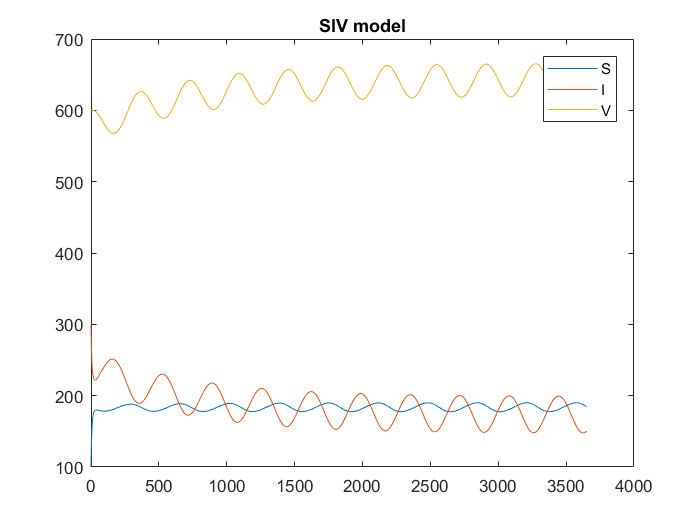
\includegraphics[scale=0.5]{../Data/sivModel_example.png}
\end{center}

Some observations: \\
\textbullet{The system tends towards a periodic equilibrium state.} \\
\textbullet{The three population subsets all vary with time, and the period is approximately one year.} \\
\textbullet{When the vaccinated population is high, the susceptible population is also high (due to more people losing immunity), and the infected population is low (due to high rate of vaccination). This matches general expectations.}

\section*{Improvement}

\textbf{Informal Notes: }I intend to fit the parameters to clinical and epidemiological data, possibly with multiple linear regression via R. I have access to data through my lab, but I would prefer to find publicly available data, possibly from the CDC.

\section*{Conclusions}

\textbf{Informal Notes: }Modeling scripts are available at https://github.com/jon-mah/SIV\_infectionDynamics

\bigskip

\bibliographystyle{mbe}
\bibliography{references.bib}


\end{document}